%
%
%
\documentclass[twoside]{wiss}

\usepackage{graphicx}
\usepackage{nidanfloat} %% appended in WISS2010 for Future Vision (2010/7/7:akita)
\usepackage{multicol}
\usepackage{here} % [H]とするとその場所に配置されるらしい
\usepackage{color}

%% balance.styを追加 (2012/9/27:watanabe, Igarashi)
\usepackage{balance}    %% 最後のページの高さを揃えるために追加  (2012/9/27:watanabe, Igarashi)
%%% 最後のページの2段組の高さを揃える.\balanceを入れる.
%%% そろえたくないときは,\nobalance


\journalhead{Babascript}

\begin{document}

\title{Babascript}
\etitle{} %2012年では英文タイトルは廃止されました.記入しないでください
% Supernavigation

\author{匿名で査読を行うため著者名なし}

\begin{abstract}

プログラムに人力処理を簡単に組み込むことのできるプログラミング環境「Babascript」を提案する。
現状のプログラムでは、コンピュータを制御することはできるが、人は制御できない。
本論文の提案手法では、通常のプログラムで関数呼び出しと同じ記法で人への処理を命令することができる。
プログラムの中に人という要素を組み込むことによって、その場の雰囲気の数値化・可視化といった
コンピュータだけでは実現出来なかったような処理を実現させることができる。

\end{abstract}

\maketitle


\section{はじめに}
コンピュータには処理が困難なタスクであっても、人ならば処理できることがある。
例えば、その場の雰囲気を数値化・文字列化することはコンピュータには処理は困難だが、人なら処理可能だ。
計算機では処理が難しいような処理を実現するために、人を計算資源として利用する手法はヒューマンコンピュテーション\cite{humancomputation}と呼ばれ、
様々な研究が行われている。

人の処理能力をプログラムから扱うことが出来れば、コンピュータだけでは実現しなかった処理を実現することができる。
しかし、既存のプログラム言語には、人に対する処理命令構文は含まれていない。
プログラムから人力処理を利用できるようにする技術は、クラウドソーシング等の分野において、研究されている(\cite{automan}, \cite{crowddb}, \cite{crowdforge}等)。
クラウドソーシングは、インターネットを経由して不特定多数の群衆にタスク処理を依頼する手法だ\cite{riseofcrowdsourcing}。

既存の仕組みでは、プログラムから人力処理を実行するためには、クラウドソーシングプラットフォームの利用が必要となる。
そのため、家族や職場の人、研究室の人たちに対してプログラムから命令を送るといったことは困難だ。
クラウドソーシングの場合、人の能力のうち活用可能なものは計算能力に限られている。
また、処理命令のための記法も複雑である。
研究事例ごとにも異なるが、クラウドソーシングプラットフォームへのアクセスキーや複雑な設定をプログラム内に記述する必要があったり、
SQL文のようなものをプログラム上に直接記述する必要があるなど、シンプルに実装することができない。

本論文では、Babascriptという、人力処理のためのシステムについて述べる。
Babascriptプログラミング環境は、関数呼び出しによって人に処理命令の通知ができるDSL Babascrtipt(図\ref{script_01})と、
Babascriptからの命令を受け取り、処理結果を入力することのできるスマートフォンアプリケーションBabascript Client(図\ref{webapp-interface})から構成される。
数行かつシンプルな人への処理命令プログラムと、スマートフォンアプリケーションによる処理命令に対する返答機能によって、人力処理を実現する。
Babascriptでは、クラウドソーシングプラットフォームを利用しない。
処理実行者はBabascript Clientというスマートフォンアプリを経由して命令を受け取る。

Babascriptを利用することで、通常のプログラムと人への処理命令をほぼ同じ記述で実現することができ、専用の記法の知識もほぼ必要ない。
シンプルな記法で人の力を借りた処理の記述が可能となる。

また、人がプログラムの処理に積極的に貢献することによって実行可能となる応用例として、
「仕事のプログラム化」と「人力による実世界プログラミング」について述べる。

\begin{figure}[!h]
  \centering
  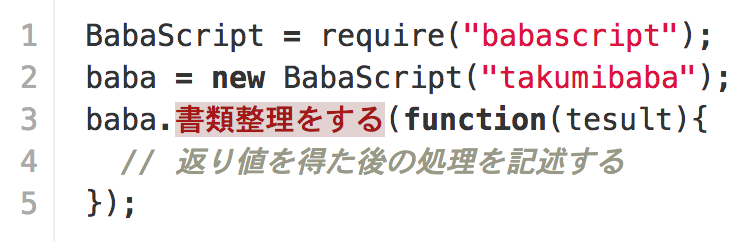
\includegraphics[width=83mm, bb=0 0 751 241]{images/script_01.png}
  \caption{Babascriptプログラム例}
  \label{script_01}
\end{figure}

\begin{figure}[!h]  
  \centering
  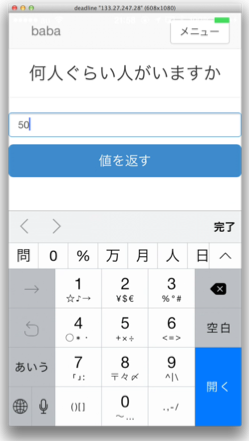
\includegraphics[width=44mm, bb=0 0 249 441]{images/interface.png}
  \caption{Babascript Clientインタフェース}
  \label{webapp-interface}
\end{figure}

\section{BabaScript}

Babascriptは、関数呼び出しによって人に処理命令を送れるDSLである。
図\ref{script_01}のようなプログラムによって、人に処理命令を送ることができる。

Babascriptは、シンプルな記法で人力処理のためのプログラムを書けるようにすることを目的としている。

\subsection{基本仕様}

Babascriptでは、定義されていないメソッドが実行されると、エラーを返さずに、人への命令構文として解釈する。
つまり、定義されていないメソッドは全て人への命令として実行され、人へと通知される。

命令の実行結果をBabascriptClientから受け取ると、関数の実行を終了し、指定したコールバック関数が実行される。
コールバック関数実行時には、引数として、処理に成功していれば、処理実行者が入力した結果が、処理失敗であればエラー文が代入されている。
人への処理命令は、通常の関数呼び出しとほぼ同じ記法で実行することができ、新たに記法を学習するといった必要がない。

人オブジェクトは宣言時にIDを指定することによって、誰に対して命令を配信するかを決定する。
例えば、id:baba に命令を送りたければ、人オブジェクト宣言時の第一引数にはbabaという文字列を指定する必要がある。
また、クライアント側でも同様に、id:baba として宣言する必要がある。

この際、指定したIDを監視するクライアントが複数人だった場合は、後述するbroadcastオプションをつかってない場合は、
命令を実行していないクライアントへと順番に配信される。

\subsection{オプション情報の付加}

人への処理命令構文の第一引数に与えるオプション情報には、返り値の型指定などの情報が考えられる。
例えばBoolean型を指定する場合には図\ref{script_02}のようなプログラムが考えられる。
他にも、指定したリストの中から値を選択してほしい、といった命令の場合は、リスト情報を格納した配列を指定する。
このオプション情報の処理は基本機能には含まれていないため、ライブラリを利用して実装する応用アプリケーションごとに対応する必要がある。

\begin{figure}[h]
  \centering  
  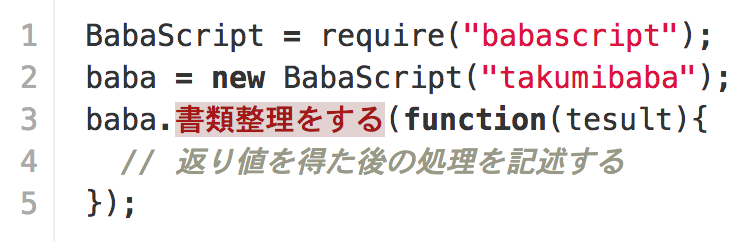
\includegraphics[width=83mm, bb=0 0 751 241]{./images/script_02.png}
  \caption{オプション情報}
  \label{script_02}
\end{figure}

特別なオプション情報として、broadcastオプションが存在する。
broadcast機能は、指定したIDを監視する全てのクライアントへとタスクを配信し、指定した数の返り値を得られると処理を終了し、コールバック関数を実行するといったものだ。

% \subsection{サンプルコード}

% \begin{figure}[h]
%   \centering  
%   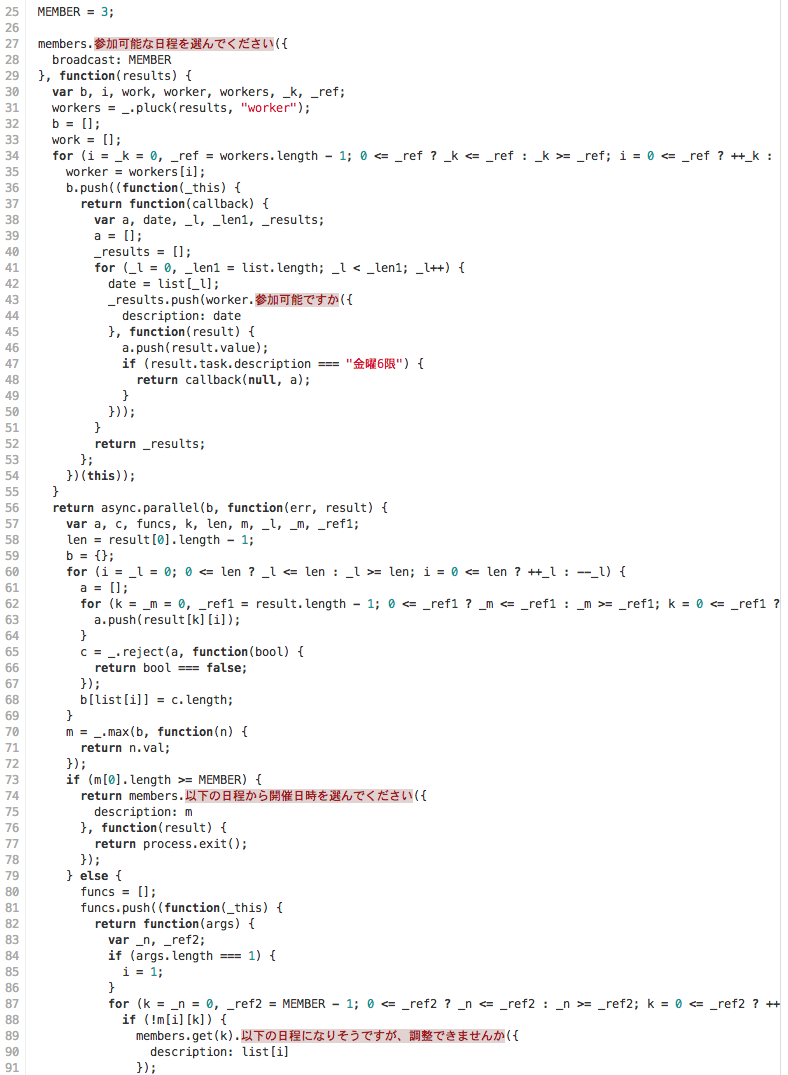
\includegraphics[width=220px]{./images/samplecode.png}
%   \caption{サンプルコード}
%   \label{sample}
% \end{figure}

\section{Babasciript Client}

Babascript Clientは、Babascriptからの命令を受け取り、値を返すためのスマートフォン向けアプリケーションである。
様々な既存のアプリケーションに人力処理のためのクライアント機能を組み込めるようにすることと、
処理実行者にとって、実行するべきことがすぐにわかって、その処理結果をすぐに返せるようにすることを目的としている。
そのため、命令を受け取る通信を行うためのライブラリ部と、返り値の入力を受け付けるUI部が分離されている。

\subsection{ライブラリ}
ライブラリ部分では、主にBabascript側との通信をおこなっている。
命令受信のイベントに対してコールバック関数を指定することで、処理命令を受け取ることができる。
基本的な利用方法は、図\ref{client}に示す。

\begin{figure}[h]
  \centering
  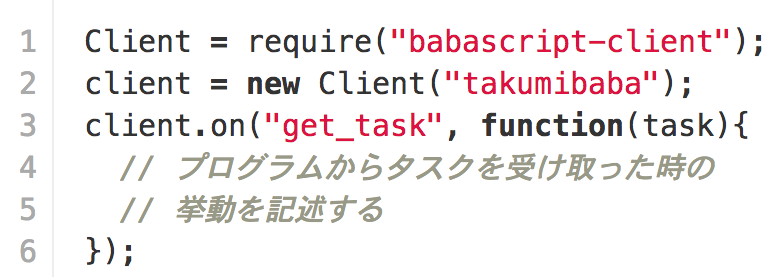
\includegraphics[width=83mm, bb=0 0 779 277]{./images/client.png}
  \caption{クライアントライブラリの基本機能 }
  \label{client}
\end{figure}

クライアントオブジェクトの宣言時、IDを指定することによって、IDに対して処理命令が発行された際にタスクを受信することができる。
また、クライアントオブジェクトが持つreturnValueメソッドを利用することで、返り値を命令発行元に返すことができる。

クライアントライブラリは、UIと完全に分離した実装となっており、かつ利用法もシンプルだ。
後述のWebアプリケーションだけでなく、様々なアプリケーションに組み込むことができる。
既存のアプリケーションであったとしても、数行のコードとUIを実装するだけである。

\subsection{Webアプリケーション}

送られてきた命令内容をユーザに提示するためのインタフェースとして、スマートフォン向けWebアプリケーションを実装した。
命令において型指定をしておくことによって、型に合った返り値を選択できるよう、ユーザに提示するUIが変化するようになっている。
例えば、Boolean型を指定していた場合、ユーザには true ボタンと false ボタンが提示され、どちらかを押すと、その結果が返り値としてプログラムに返される。

スマートフォンに最適化したWebアプリケーションとして実装しており、様々な場面において利用可能だ。
実世界におけるタスクを処理しながらでも十分に利用可能である。
図\ref{webapp-interface}のような画面を持つ。

\section{実装}

上記システムは全てJavascriptで実装した。
Babascript はNode.js上で動作し、Babascript ClientはWebブラウザ上で動作する。
全体図は図\ref{system}のとおりだ。

\begin{figure}[h]
  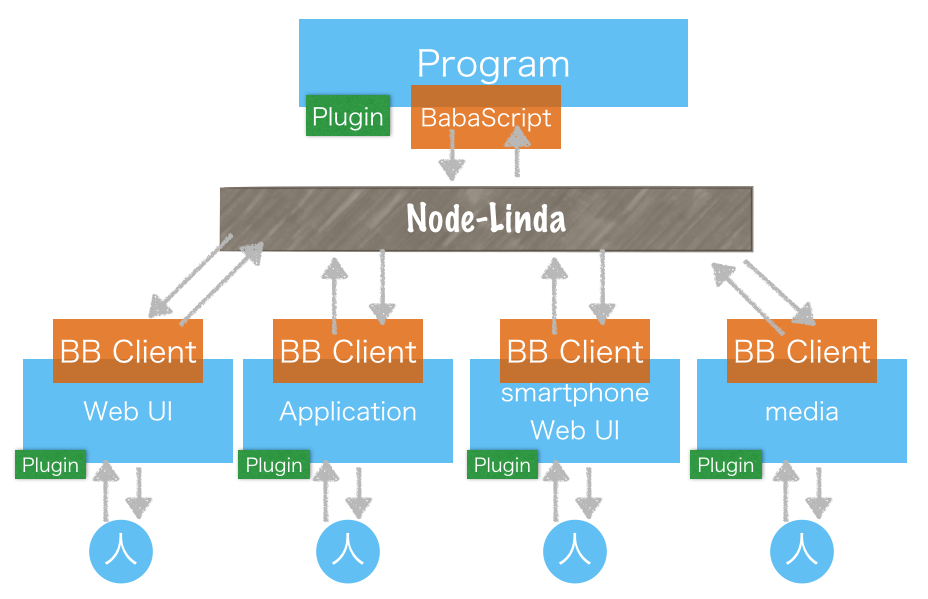
\includegraphics[width=83mm, bb=0 0 928 599]{./images/system.png}
  \caption{システム全体図}  
  \label{system}
\end{figure}

BabascriptとBabascriptClient間の通信を実現するために、Node-Linda\cite{linda}を利用した。

\subsection{処理の流れ}

Babascriptは、以下のようなフローで人への命令構文が実行される。

1. 人への命令構文を実行する
2. 命令がNode-Lindaサーバを経由してクライアントへと配信される
3. 命令を受け取ったクライアントがユーザに処理を促す
4. 命令実行者が、処理結果をBabascriptClientに入力する
6. Node-Lindaサーバを経由して実行元プログラムに入力された処理結果が送信される
7. プログラム側で、指定されたコールバック関数が実行され、処理が続く

\subsection{タスク情報の構成}

人への処理命令構文の実行によってタスク情報が生成される。
このタスク情報は、図\ref{task}のようなjsonオブジェクトとなる。

\begin{figure}[!h]
  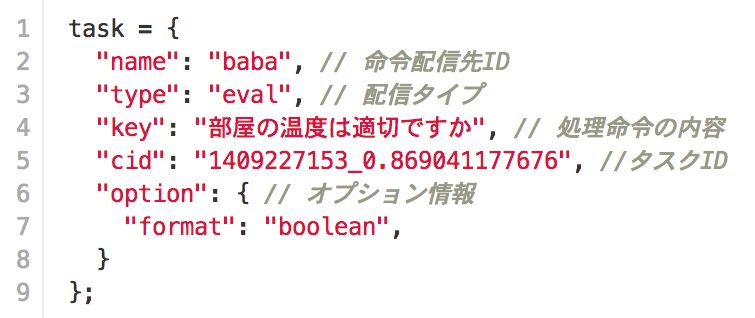
\includegraphics[width=83mm, bb=0 0 755 318]{./images/task.png}
  \caption{タスクのJSONオブジェクト}  
  \label{task}
\end{figure}

\section{応用例}

以下のような応用が考えられる。

\subsection{仕事のプログラム化}
みでもできてしまい、部分部分で人の意思や感性、知識を加えるだけで良い -->

人への命令がプログラムとして記述可能になることで、人の仕事をプログラム化することができる。
人の仕事は、例えば、マニュアルのような形で記述されることが多い。
マニュアルで全て記述できるような場合は、Aという条件の時にはBの処理を実行する、
といったことが文章として記述されていることが多く、その内容の多くはプログラムのようなものであるため、プログラム化は可能であると言える。

プログラム化し、実行することによって、状態をプログラムによって管理することが可能となる。
つまり、条件判断や記憶が必要なことは出来るだけコンピュータ側に処理させる、といったことが可能になる。
人は細かい条件などを覚えておいたり、自分で判断することなく、ただ指示されたことのみを実行することで、仕事を終わらせることができるようになる。
ただ指示されたことのみを実行するだけで良いならば、仕事の引き継ぎなども必要なくなり、人の代替も容易となる。

また、人同士がコミュニケーションを取ることなく、複数人を協調させるといったことも可能となる。
通常、複数人を協調させるためには、人同士が相談したり、上位の意思決定者が必要となる。
しかし、コミュニケーションはコストのかかるものであり、適切に行われない場合、問題が生じることもある。
意思決定をプログラムに委ねることは、複数人を効率よく協調させることに繋がるとも考えられる。

全ての仕事をプログラム経由にすることで、詳細な実行ログや実行状況を把握することもできる。
仕事の実行量の定量化や、状況監視、状況の可視化などに活かすことができる。

\subsection{人力による実世界プログラミング}

人をセンサーやアクチュエータとして利用することで、人によって実世界を操作する実世界プログラミングが可能となる。
現在のセンサーやアクチュエータでは、実世界に干渉するのには限界がある。
例えば、その場の雰囲気を数値化したり文字列化するといった、コンテキスト情報を伴ったセンシングは困難である。

しかし、人力処理を組み込むことのできる本提案手法ならば、コンテキスト情報を伴うようなセンシングであっても、実現可能である。
また、人を汎用的に利用可能なアクチュエータとして利用することもできる。
人をセンサーとして扱う Human as Sensor、人をアクチュエータとして利用する Human as Actuator の両者を組み合わせることによって、
より柔軟に実世界へと干渉可能なプログラミングが可能となる。

また、本提案手法では通常のプログラムと人力処理のプログラムを混合させることができるため、
条件次第で人とコンピュータのどちらに処理させるかをプログラムが判断し、適切な方に処理させるということも可能である。

\section{考察}

Babascriptについて、以下のように考察する。

\subsection{人がプログラムの処理に貢献する}

プログラムは、コンピュータの能力を利用して人を支援するためのものであり、人が積極的にコンピュータの能力を補うものではなかった。
コンピュータで実行可能であるならば、コンピュータで実行するのが良い。
しかし、人にしか出来ないことも現在の技術では存在する。
そこで、処理の実現を諦めるのではなく、コンピュータが得意なことはコンピュータが、人が得意なことは人がやるようにすれば良い。
技術がないから諦めるのではなく、人という要素を積極的に利用すれば、むしろ全体的な処理の正確性の向上や高速化に寄与する可能性もあるのではないかと考える。

\subsection{命令を受ける処理単位としての人}

本研究では、人は処理を命令され実行するノードとなり、プログラム上においてコンピュータやセンサーと同等となる。
こういったことに対して心理的な拒否感を覚えることも考えられる。
しかし、一処理ノードとして扱うことによって、大きなメリットもある。
命令を実行するだけのノードであるということは、ただ処理内容を実行することにのみ集中すれば良いということだ。
ただやるべきことだけが提示され、その通りに動けば良いということは、深く考える必要がなくて楽であるということが考えられる。
もちろん、全ての処理がただ提示する通りに動けば良いものではないが、作業を楽にするための一つのアイデアであると言える。

\subsection{タスク実行の遅延と実行保障性}

Babascriptによってタスク実行を依頼しても、人がすぐにタスクを実行し値を返すことを完全に保証することはできない。
タスク受信端末を見ていない、受信しても実行できないといった状況の場合、すぐに値を返すことはできない。
この際、Babascriptによる処理が原因で全体の処理が遅延する可能性がある。

また、労働関係にあるなど、タスク実行に強制力がある場合は、タスク実行が確実に行われると考えられるが、強制力がない場合はそもそもタスク受信を無視するといったことも考えられる。
タスク実行に強制力がない場合は、金銭などのインセンティブを与えるといった手段によって、実行保障性を確保するといったことが考えられる。

\subsection{例外処理}

Babascript環境において、命令文と現実との乖離によって適切な返り値を選択・記述ができなくなるといった可能性がある。
これは、現実が刻々と変化していることなどから、完全に避ける事の出来ない問題であると考える。
この際、無理やり値を返すといった処理をしてしまうと、本来の状態とは違った判断がなされてしまう危険性がある。
命令文とは明らかに現実が異なっている場合などは、タスク実行者から例外としてプログラムに通知出来るような仕組みの実装によって、問題の解決へと繋げられると考える。

\subsection{命令内容の粒度}

Babascriptでは、タスクの命令文の記述には制限がないため、自由となっている。
抽象度が高すぎる命令は、あいまいな表記となり、タスク実行者にとって理解しづらい文面となり得る。
その結果、想定外の処理が実行され、意図しない結果を招く恐れがある。
抽象度が低すぎる命令は、全体の処理内容にもよるが、プログラム自体が冗長となり得る。
プログラムとタスク実行者の間のやりとりが増え、通信や待機時間などがボトルネックとなる可能性がある。
また、タスク実行者にとっても、やりとりが増えることで負担増になると考えられる。
処理ごとに異なると考えられるが、命令文は適切な抽象度に設計しなくてはならない。

\subsection{複数命令の同時実行}

複数のプログラムから同時に一人のタスク実行者へとタスクが配信される可能性がある。
この際、異なるコンテキストにある命令が交互に配信され、タスク実行に大きな障害をもたらす可能性がある。
例えば、料理プログラムと掃除プログラムが同時に実行された場合、鍋で煮ている途中で「洗剤を投入しろ」などといった命令が配信されることが考えられる。

この問題は、全てのBabascriptプログラム中において、一人のタスク実行者は一つのプログラムからのみ、連続してタスクを受信できるような仕組みを用意することによって、解決可能であると考えられる。
また、応用アプリケーションでの実装になるが、コンテキストを明示し、どの処理系におけるタスクなのかをタスク実行者に示すといった手段によっても解決可能である。

\section{関連研究}

計算機では処理が難しいようなタスクを解決するために、人を計算資源として利用する手法はヒューマンコンピュテーション\cite{humancomputation}と呼ばれ、様々な研究が行われている。
インターネットを介して不特定多数の群衆にタスクを実行させるクラウドソーシングと組み合わせた研究事例も多く存在する。
クラウドソーシングのプラットフォームとしては、Amazon Mechanical Turk\cite{mechanicalturk}が存在する。
Barowy らは、CrowdProgrammingという概念を提唱し、プログラミング言語内においてクラウドソーシングによる計算とコンピュータによる計算の統合を実現した\cite{automan}。
Franklin らは、機械だけでは答えられないようなDBへのクエリに対する応答を、クラウドソーシングを用いることで返答可能にするCrowdDBを提案している\cite{crowddb}。
Morishima らは、人をデータソースとしてプログラムの中で利用する手法を提案している\cite{cylog}。
crowdforge-->
これらの研究では、クラウドソーシングを利用した問題解決手法の提案をしている。
本研究は、不特定多数の群衆をプログラムするためのものではなく、実世界の操作なども含むため、家族や職場の人のような特定可能な人物を対象としている。
また、人を計算資源やデータソースとしてシステムに組み込むことを前提としているが、本研究は、計算資源やデータソースに限らず、実世界への干渉等も対象としている。
本研究はより汎用的な枠組みであると言える。

ユビキタスコンピューティングの研究分野においては、Human as Sensorという概念も提唱されている。
PRISMは、スマートフォンを利用したセンシングプラットフォームだ\cite{prism}。
Liuらは、ソーシャルメディア上の人をセンサーとして扱ったQ\&AサービスMoboQを提案し、その検証を行った。
Human as Sensorに類する研究では、人をセンサーとして扱うことを対象としているが、本研究ではセンサーのみを対象としていない。

Chengらは、モーションプラットフォームにおけるモーターやメカニカル機構の代替として人を利用したHaptic Turkを提案している\cite{hapticturk}。
Haptic Turkはゲームでの利用に特化したものだ。
本研究は、用途を限らない汎用的な仕組みとなっている。

加藤らは、人とロボット間でのタスク共有システム Sharedoを提案した\cite{sharedo}。
人とロボットのタスク実行における協調は、本研究の主眼である「何かの処理を実現するとき、人とコンピュータは相補的に動作するべき」という考えと大きく類似している。


\section{おわりに}

本論文では、プログラムに人への処理命令を組み込むことのできるプログラミング環境 Babascript を提案した。
人をプログラムに組み込み、制御できるようにすることで、

何かの処理を実行していく上で、コンピュータにできることは極力コンピュータに処理させ、人は人にしかできないことや、人がやるべきことだけを処理するというのが本来あるべき処理の切り分け方であるが、現状ではその切り分け方はあいまいである。

Babascriptによって、人はプログラム上においてコンピュータと同じ処理ノードとして存在し、関数実行によって処理内容を受け取り、実行して値を返す存在になれる。
これによって、プログラマブルになりつつある世界において人自身もその一部になることが可能となる。

また、Babascript環境によって実現する応用例を示すことによって、人をプログラマブルにした際のメリットを示した。

今後は、議論で述べたBabascriptの問題点などを改善していく。


{\scriptsize
\bibliographystyle{jwiss}
\bibliography{paper}
}

\end{document}


